\section{Phase 0 Mathematical Framework}
\label{sec:method}

\subsection{Intraday Cost-of-Carry Factorization and Discrete Hedging}
\label{sec:method_carry}

Consider a synchronized continuous-matching grid of 225 minutes per trading day across 250 trading days per year, where each 5-minute bar has duration $\Delta = 5$ minutes and annualized step $\Delta_{\mathrm{year}} = 1 / 11{,}250$ years. At bar $n$, let $F_n > 0$ and $S_n > 0$ denote the closing levels of \texttt{VN30F1M} (contract multiplier $100{,}000$ VND/point) and \texttt{VN30INDEX}. Under both continuous dividend yields and discrete cash-dividend schedules, exact cost-of-carry parity admits an affine factorization with zero analytical residual, while log-basis decomposition incurs a strictly bounded higher-order remainder.

When projecting futures price changes onto discrete rebalance intervals of step $\Delta$, the discrepancy between discrete-time minimum-variance hedging and continuous-time instantaneous projection obeys an exact rational formula whose leading asymptotic term scales linearly as $O(\Delta)$. Furthermore, evaluating Ornstein-Uhlenbeck mean-reversion weights over short intraday intervals via naive $1 - \exp(-x)$ suffers catastrophic subtractive cancellation as dimensionless stiffness $x = \kappa_n \Delta \to 0$; evaluating $-\operatorname{expm1}(-x)$ eliminates cancellation down to machine epsilon.

\subsection{Dynamic Market Hypergraph Spectrum and Admissibility}
\label{sec:method_hypergraph}

At each 5-minute bar $n$, we represent synchronous multi-asset couplings over the $M$-node market universe $\mathcal{V}$ as a time-indexed weighted hypergraph $\mathcal{H}_n = (\mathcal{V}, \mathcal{E}_n, \mathbf{W}_n)$ with non-negative incidence matrix $\mathbf{H}_n \in \mathbb{R}^{M \times E_n}$ and diagonal hyperedge weight matrix $\mathbf{W}_n$. Letting $\mathbf{D}_{v,n}$ and $\mathbf{D}_{e,n}$ denote the diagonal vertex and hyperedge degree matrices, the symmetric normalized propagation operator $\mathbf{S}_n \in \mathbb{R}^{M \times M}$ and normalized hypergraph Laplacian $\boldsymbol{\Delta}_n \in \mathbb{R}^{M \times M}$ are defined by
\begin{equation}
  \mathbf{S}_n = \mathbf{D}_{v,n}^{-1/2} \mathbf{H}_n \mathbf{W}_n \mathbf{D}_{e,n}^{-1} \mathbf{H}_n^\top \mathbf{D}_{v,n}^{-1/2},
  \qquad
  \boldsymbol{\Delta}_n = \mathbf{I}_M - \mathbf{S}_n.
  \label{eq:hypergraph_laplacian}
\end{equation}
By congruence with a contraction, every eigenvalue $\lambda$ of $\boldsymbol{\Delta}_n$ lies in $[0, 1]$, preventing spectral explosion across stacked message-passing layers. Downstream parameter heads apply smooth order-preserving transformations that enforce hard economic admissibility bounds identically, as summarized in \Cref{fig:pipeline}.

\begin{figure}[t]
  \centering
  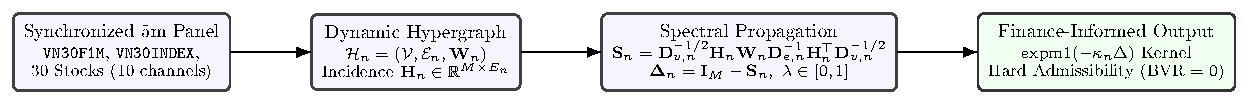
\includegraphics[width=0.98\linewidth]{fig_rc_fihgnn_pipeline.pdf}
  \caption{Phase 0 RC-FIHGNN data-to-admissibility pipeline mapping synchronized 5-minute futures, index, and 30-stock order-flow channels through dynamic hypergraph incidence, normalized spectral propagation, and hard economic admissibility projection.}
  \label{fig:pipeline}
\end{figure}
